\subsection{21 августа. Т/б <<Глобус>>}

\textit{Метеоусловия: утром, днём, вечером ясно, тепло}


\begin{figure}[h!]
	\centering
	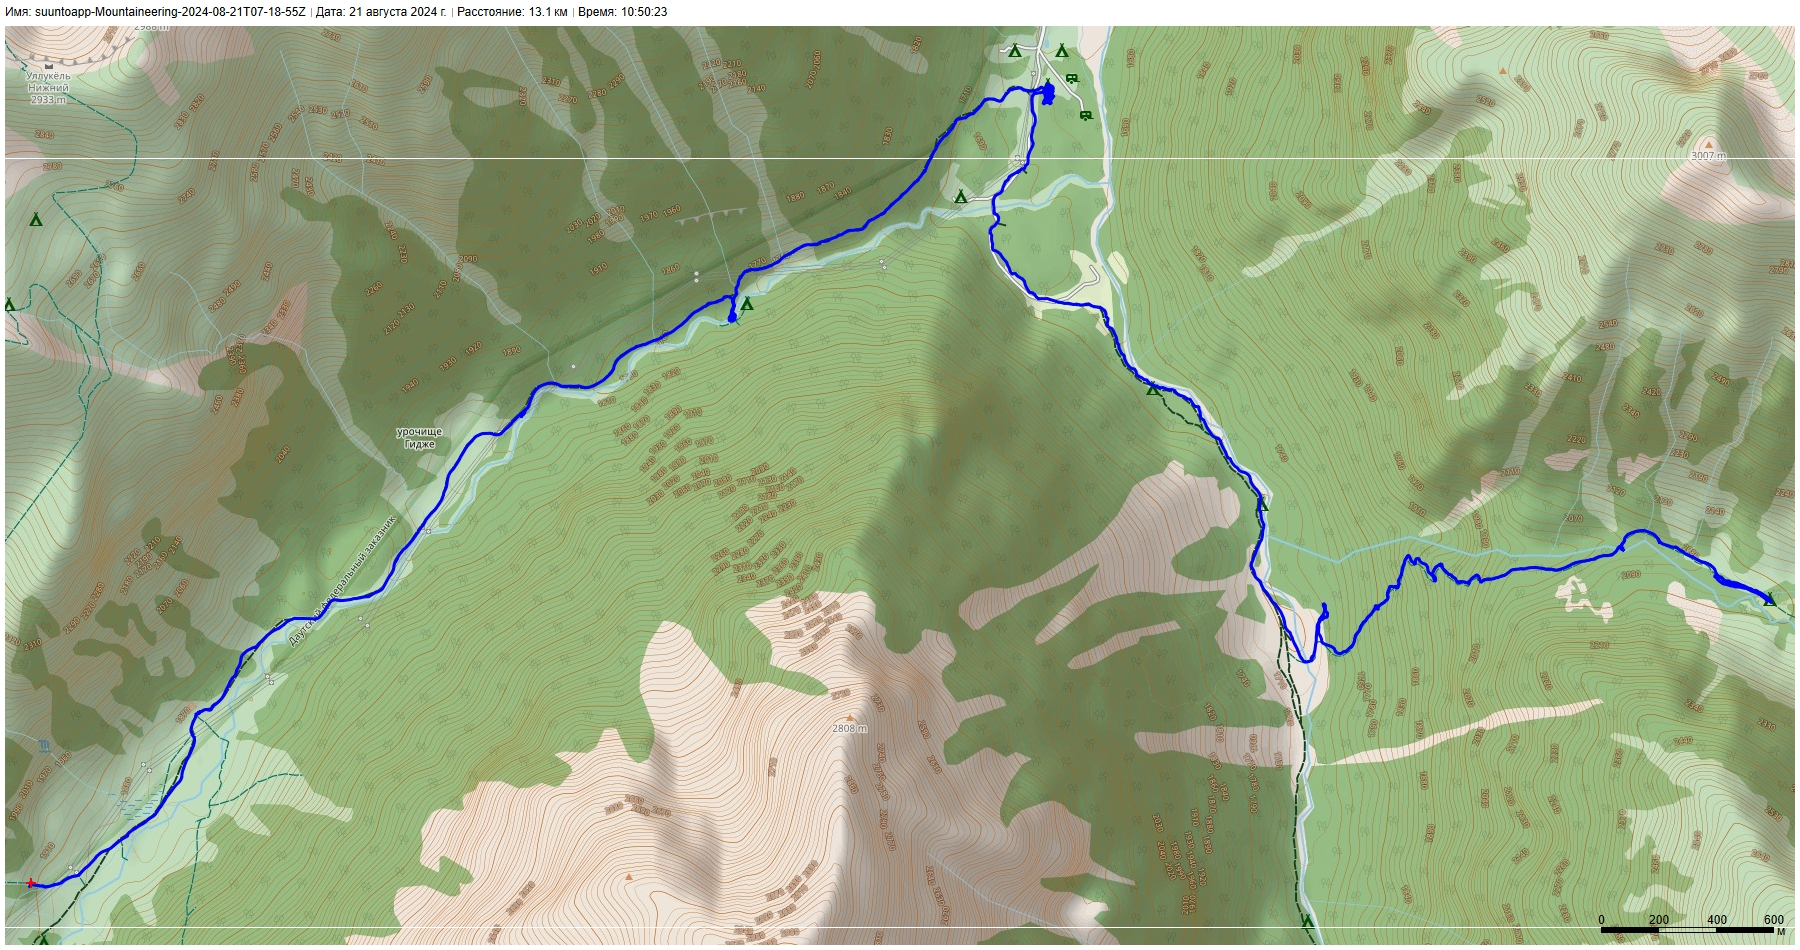
\includegraphics[angle=0, width=0.7\linewidth]{../pics/mini_maps/21}
	\label{fig:mini_21}
\end{figure}

Встали х/з во сколько, ибо, раз не будили, значит проснулся сам. Почивать завтраком меня изволили чем-то непримечательным, потому что не запомнилось. Какао, свежей дичи или пирога с угрями не подавали. Кроме того, раз завтрак не запомнился, я ещё и не был дежурным. Это прекрасно.

Омрачался мой лик лишь резкой пульсацией боли в левом ухе – подцепленный в поезде отит не желал меня отпускать. Но этот пустяк был быстро нивелирован торжественным вручением <<Нурофена>> нашим медиком (вернее, помощью в его самостоятельном применении, разумеется, мы помним базовые принципы ПП), у которого ещё с предыдущего дня продолжали стекать капельки крови с травмированной руки. Попытка нашего медика прорубить проход в перевале для уставшей группы одним резким ударом ледоруба в полёте с ледника достойна воспевания в сагах, хотя именно после неё я задумался о том, чтобы-таки пройти все курсы <<Вершины>>, на случай, если первая помощь в течении похода будет нужна только медику.

С утра место нашей стоянки производило в высшей степени благоприятное впечатление, которое резко контрастировало с тем, что было, когда мы на него пришли в ночи вчера, освещая фонариками беспечную физиономию руковода-сан. Небольшой участок леса с живописной журчащей речушкой, старыми, покрытыми мхом камнями и брёвнами.

Самый важный приём пищи я осуществлял с видом на этот пейзаж на камушке, возвышавшемся на внушающем мимолётные суицидальные мысли обрыве. Обрывчике.

Крайне неспешный приём пищи, мыльно-рыльные мероприятия и сборка лагеря весьма одухотворили и подготовили меня к новым подвигам. Из подвигов сегодня ожидалось посещение турбазы «Глобус», пребывание на этой базе, а затем прогулка с рюкзаком к началу долины до следующего перевала. 

Другие участники также были, в целом, довольны обстановкой. Впрочем, не могу не отметить, что Георгия явно утомили его «доспехи», изготовленные собственноручно руководителем группы, и он поспешил от них избавиться. Стратегия Георгия вообще явно выходила за горизонт планирования…

Итак, собрались, оделись, умылись, спрятали айфоны в гермочехлы, свернули свои косметички, подтянули корсеты, проверили фижмы под юбками – всё в порядке, группа из Москвы выдвигается до турбазы. 

Дорога предстояла нелёгкая – вместо асфальтированного хайвея предстояло преодолеть где-то 5 км по грунтовке, причём по дороге не было ни одной кофейни, и негде было наполнить бутылки смузи.
Прекрасные виды, остановки для селфи и хеви-метал в наушниках внушали надежды на позитивный исход нашего мероприятия. Мысли мои были где-то вдалеке от этих мест, я был погружён в размышления о перспективах развития хоббихорсинга среди конной полиции, о том, какую магию разрешено использовать в борделях вселенной «Гарри Поттера», а также о том, являются ли конфеты с коньяком каноничным блюдом для бранча.

Также я нашёл себе ещё одно развлечение на весь поход – периодически спрашивать у руковода (в юности имевшего репутацию биолога среди одноклассников) «чо за ягода». Серьёзным испытанием стала крупная ягода ярко оранжевого цвета, обнаруженная среди неспелой брусники, сходу опознать которую не удалось. Титаническим усилием шейных мышц руковода было установлено, что это упавшая с дерева рябина.

К великому удовольствию всех участников, наша сомнительная компания показалась пограничникам на заставе абсолютно безобидной, так что товарищи командиры отпустили нас с миром. 
Дальнейший поиск истин был прерван прибытием на источник нарзана с природной газацией. Это было просто наслаждение, там ещё и живописный мостик через бурную горную речку. В нарзан, естественно, мы бахнули аскорбинки.

Обретя таким нехитрым образом высшую степень блаженства, мы благополучно дошли до турбазы – погода была солнечная, ясная. Никаких приключений.

Турбаза «Глобус» должна была стать местом сытного обеда. Кроме того, на неё надо было забрать часть «заброски». 

Из особенностей хочется отметить сравнительно демократичные цены в магазинах, настойчивое желание местных продать хичыны всем прибывшим, а также ощутимое нежелание предоставлять вай-фай даже для чрезвычайных нужд. А нужда, как оказалось, была…

Вскоре по прибытию наш руковод предложил Георгию «отойти поговорить». Так страшно мне не было даже во время обвала в пещере. Для разговора руковод выбрал полянку метрах в пятидесяти от основной стоянки, видимо, из расчета на то, что другие участники группы не должны слышать суть разговора, но должны видеть, что их ждёт в случае чего. Fear me, but follow.
Таких резких движений руками и ногами, кои осуществлял наш руковод во время «разговора», я не отрабатывал даже на занятиях по ММА. Даже на предложения присесть в группе реагировали как-то неуверенно. Как-то на было ногах спокойнее.

«Разговор» окончился тем, что Георгий (принимающая сторона беседы) выступил с публичным заявлением: он заявил о принятии решения сойти с маршрута и отправиться домой.

Опуская смехупочки, объективные причины для такого решения были: откровенно неудачный выбор «снаряги» (у человека не было нормальной одежды, правда, была косоворотка), боли и странные новообразования в коленях, общие проблемы физической подготовки и прочее (я не знаю, куда именно отнести решение нести в походе 4 книги и коробку с игрой в <<го>>).

Руководы поставили задачу – найти связь (ибо через трекер это было медленно). Я взял в охапку всех девчонок, что были не заняты, т.к. иначе мне скучно, и пошёл колесить по соседним турбазам (а они в шаговой доступности). На втором круге мы зашли внутрь, где я случайно разговорился с каким-то дедушкой, который оказался боссом и хозяином нескольких турбаз. За 300 рублей он согласился дать позвонить куда надо и кому надо, а также предложил самостоятельно отвезти кого надо куда надо. Дальше я связал руковода и дедушку-босса и вопрос с отправкой Георгия домой всецело лёг на узкие плечи нашего походного начальника Дарьи <<фонарики-далеко-не-убираем>> Снеговской.

Выдалась ситуация неопределённого объема свободного времени, который был потрачен поистене рационально. Например, я помогал Алексею (супруг руковода и фактически второе лицо в государстве походе) время от времени вытаскивать солнечную батарею из тени на солнце. Мы успели кучу всякого зашить-починить-подзарядить. Короче, четвертый день – а мы уже большие молодцы.

Смеркалось. Трансфер для Георгия был подан, и после краткого прощания группа, глядя на удаляющийся автомобиль, осознала, что чилл закончился и теперь придется куда-то переть наши замечательные рюкзаки.

Руковод Дарья твердо и чётко утверждала, что переход до места ночёвки планируется небольшой (пара километров) и по дороге. Затем группа встает у реки, где начинается заход в нужную долину и готовится спатинькать.

Вроде бы как, всё логично, ведь группа днём ранее завершала спуск с перевала с фонариками, матюками и голыми сиськами. Зачем повторять ненужные подвиги. 

Однако «твёрдо и чётко» — это прямая отсылка. До нужной точки мы дошли. Тут всё хорошо. А вот дальше…

Уже на месте, руковод вдруг начал рассказывать душераздирающую историю о том, как они шли по этому маршруту 6 лет назад, дошли до этого места, начали подниматься, поднялись на 300 метров, стемнело, пришлось спускаться и ставить лагерь, а на следующий день выяснилось, что они не дошли всего ничего.

Но теперь-то, утверждал руковод, всё будет по-другому! Да, придётся подниматься по лесной тропе 300 метров с фонариками, но теперь-то мы знаем, где и как стоять (конечно, ведь мы в ночи легко опознаем то место, которое видел один человек при свете дня шесть лет назад).

Предлагалось, в общем, руководом совершить подъём, 
и поставить лагерь. А я же молодец, я взял себе рюкзак 35 кг, мол, знаю же, что идти всего пару километров по прямой. А тут на тебе – десерт. Кушай изотоник, не обляпайся, допивай свой нарзанчик, если что-то не так – то знай, что тебе кажется. Ведь, в итоге, нашу 
цель на сегодняшний вечер нельзя было назвать нереальной.
Именно тогда я научился смотреть матом, а первые буквы абзаца выше совершенно случайно сложились в слово, являвшееся эпиграфом в сложившемся моём мнении о происходящем.
Впрочем, мы дошли, поставили лагерь и легли спать. С погодой везло весь день, но глазик начал дёргаться. И это был только четвёртый день.


\begin{figure}[h]
	\centering
	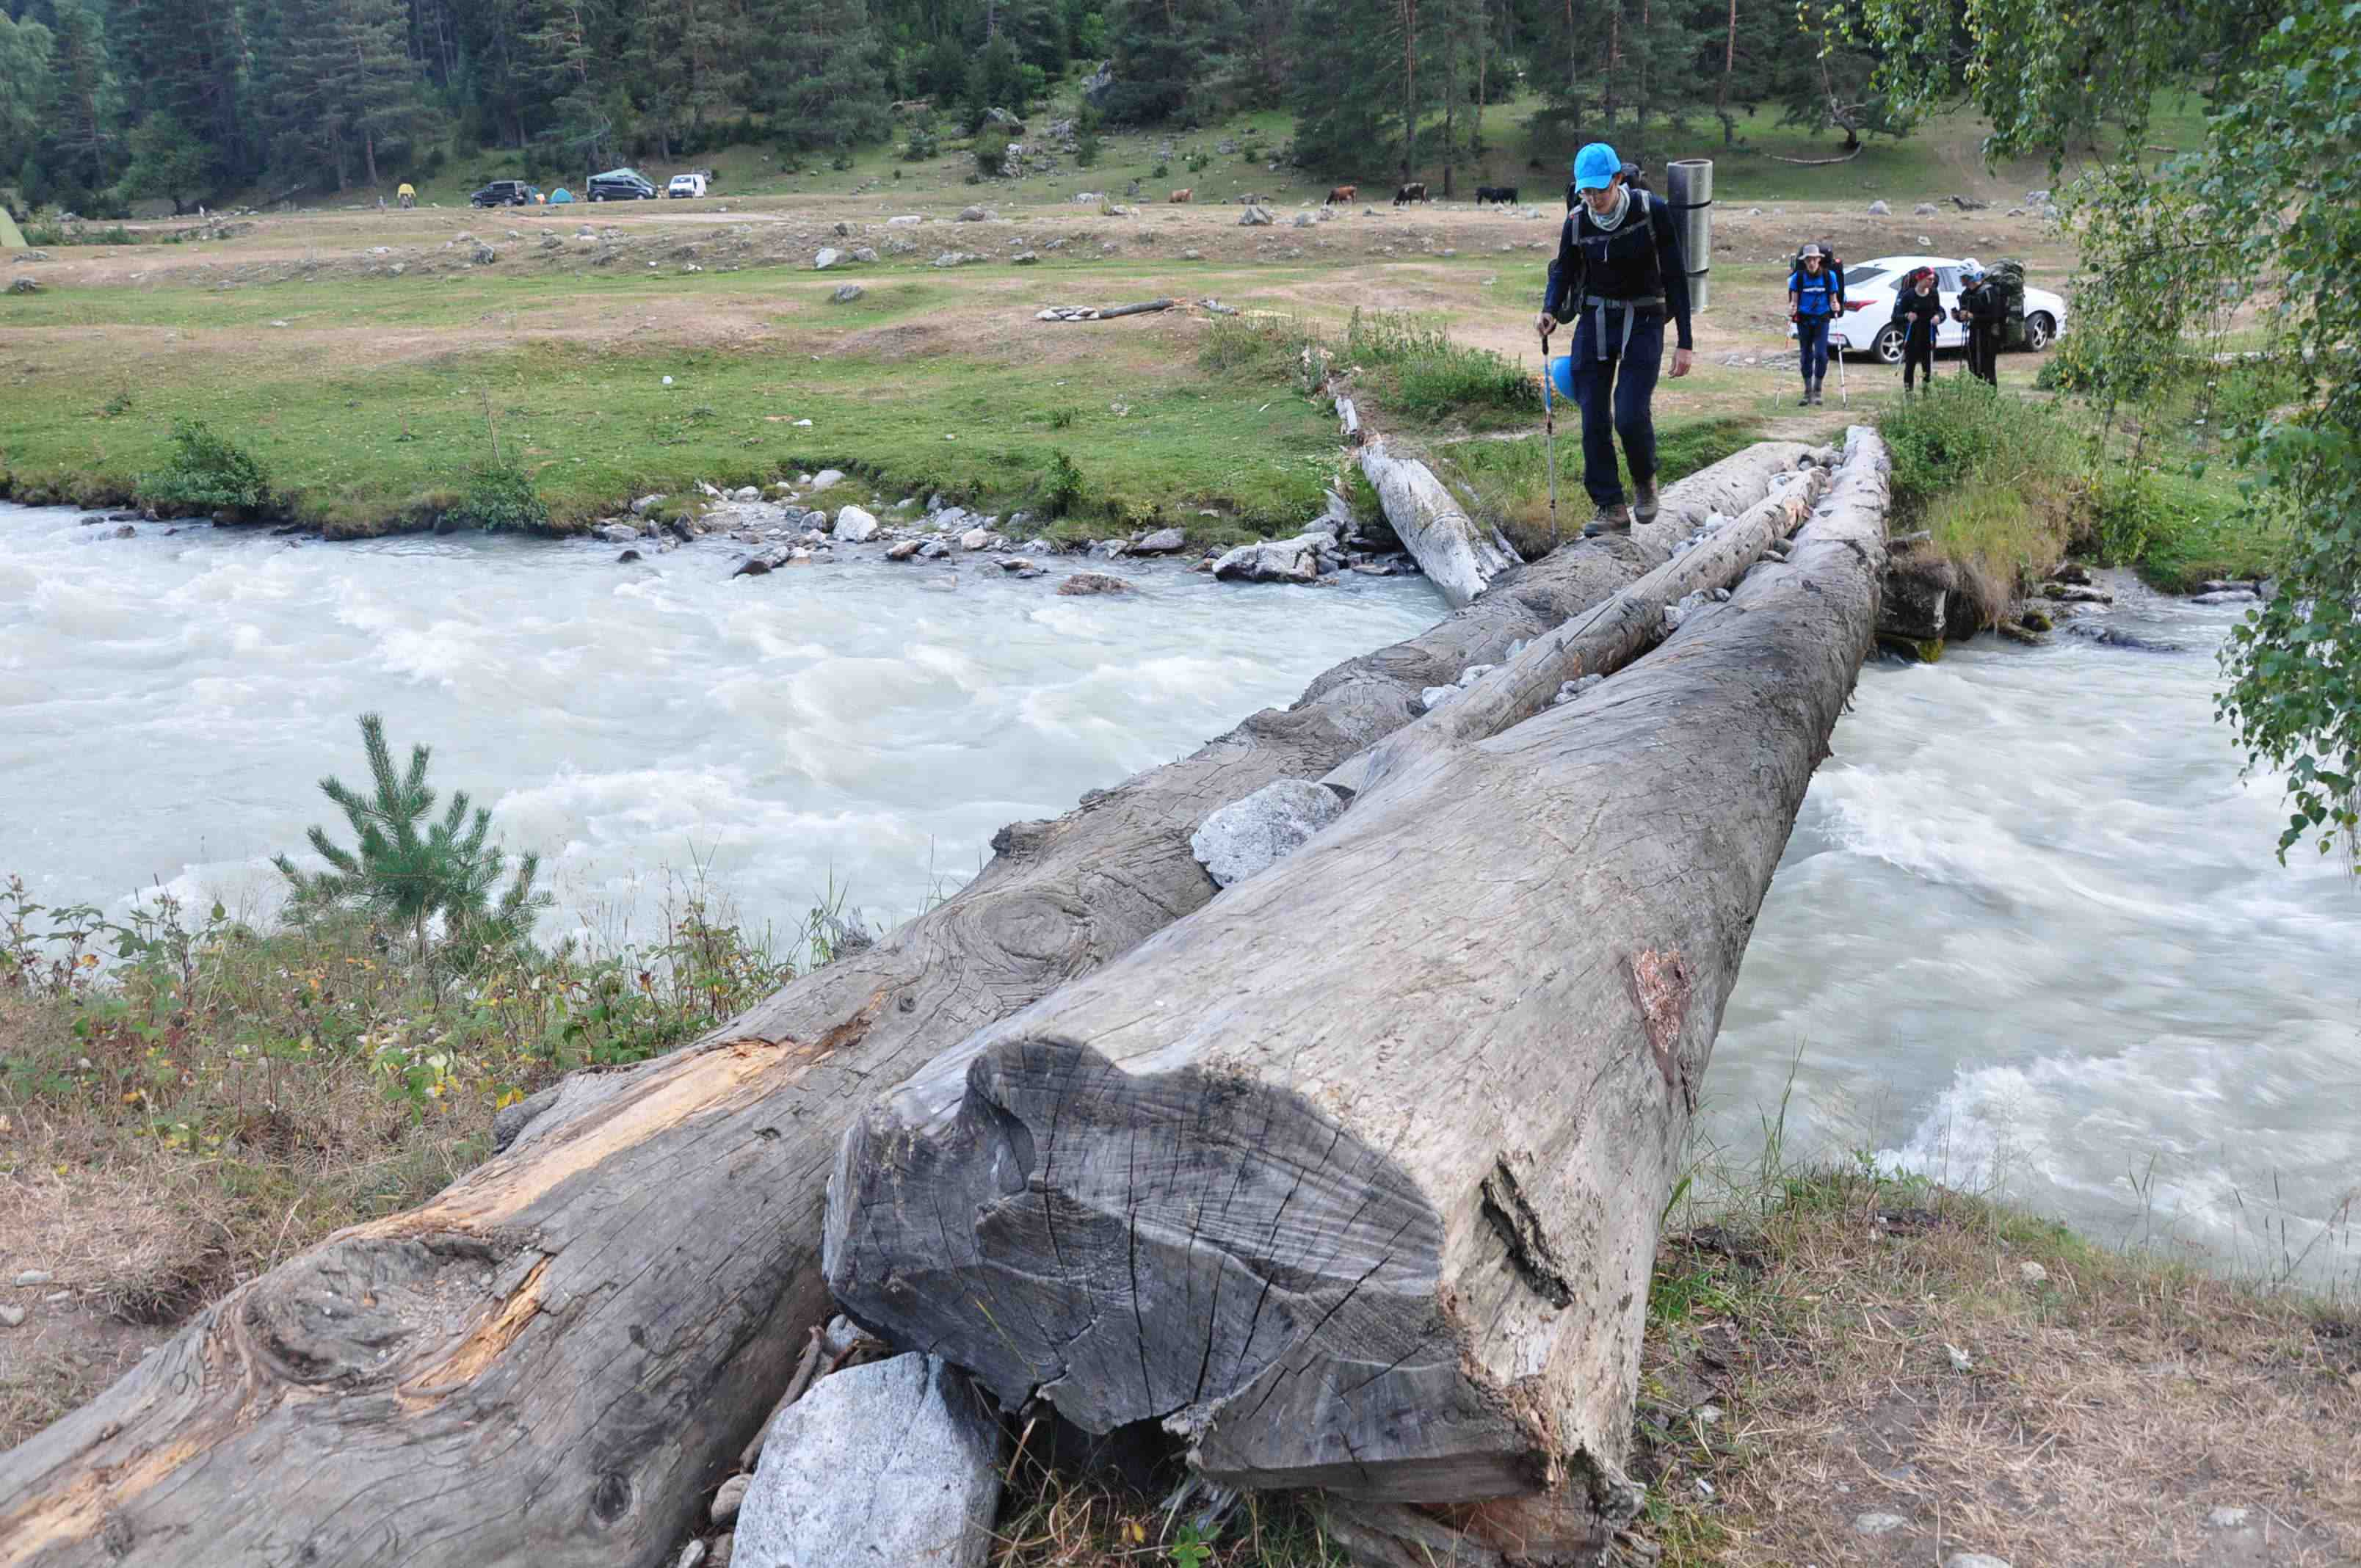
\includegraphics[width=0.7\linewidth]{../pics/DSC_1167}
	\caption{Группа пересекает р. Гондарай по мосту из бревён}
	\label{fig:hondaray}
\end{figure}
\newpage